\documentclass{article}
\usepackage{ae,aecompl}
\usepackage{todonotes}
\usepackage{chngcntr}
\usepackage{tikz-cd}
\usepackage{graphicx}
\graphicspath{ {./images/}}
\usepackage[all,cmtip]{xy}
\usepackage{amsmath, amscd}
\usepackage{amsthm}
\usepackage{amssymb}
\usepackage{amsfonts}
\usepackage{bm}
\usepackage{qsymbols}
\usepackage{latexsym}
\usepackage{mathrsfs}
\usepackage{mathtools}
\usepackage{cite}
\usepackage{color}
\usepackage{url}
\usepackage{enumerate}
\usepackage{verbatim}
\usepackage[draft=false, colorlinks=true]{hyperref}
\usepackage{pdfpages}
\usepackage[margin=1.2in]{geometry}
\usepackage{IEEEtrantools}

\usepackage{fancyhdr}


\usepackage[nameinlink]{cleveref}


\DeclareMathOperator*{\ac}{accept}
\DeclareMathOperator*{\amax}{argmax}
\DeclareMathOperator*{\amin}{argmin}
\DeclareMathOperator*{\Aut}{Aut}
\newcommand {\al}{{\alpha}}
\newcommand {\abs}[1]{{\left\lvert#1\right\rvert}}
\newcommand {\A}{{\mathcal{A}}}
\newcommand {\AM}{{\mathrm{AM}}}
\newcommand {\AMp}{{\AM_{p}^{X}\!(\Ri_\w)}}
\newcommand {\B}{{\mathcal{B}}}
\DeclareMathOperator*{\Be}{Bern}
\newcommand {\Br}{{\dot{B}}}
\newcommand {\Ba}{{\mathfrak{B}}}
\newcommand {\C}{{\mathbb C}}
\newcommand {\ce}{\mathrm{c}}
\newcommand {\Ce}{\mathrm{C}}
\newcommand {\Cc}{\mathrm{C_{c}}}
\newcommand {\Ccinf}{\mathrm{C_{c}^{\infty}}}
\DeclareMathOperator{\cov}{Cov}
\DeclareMathOperator{\DEV}{DEV}
\newcommand {\Di}{{\mathbb D}}
\newcommand {\dom}{\mathrm{dom}}
\newcommand{\dist}{\stackrel{\mathrm{dist}}{=}}
\newcommand {\ud}{\mathrm{d}}
\newcommand {\ue}{\mathrm{e}}
\newcommand {\eps}{\varepsilon}
\newcommand {\veps}{\varepsilon}
\newcommand {\vrho}{{\varrho}}
\newcommand {\E}{{\mathbb{E}}}
\newcommand {\Ec}{{\mathcal{E}}}
\newcommand {\Ell}{L}
\newcommand {\Ellp}{{L_{p}[0,1]}}
\newcommand {\Ellpprime}{{L_{p'}([0,1])}}
\newcommand {\Ellq}{{L_{q}([0,1])}}
\newcommand {\Ellqprime}{{L_{q'}([0,1])}}
\newcommand {\Ellr}{L^{r}}
\newcommand {\Ellone}{{L_{1}([0,1])}}
\newcommand{\Elltwo}{{L_{2}([0,1])}}
\newcommand{\Ellinfty}{L^{\infty}}
\newcommand{\Ellinftyc}{L_{\mathrm{c}}^{\infty}}
\newcommand{\exb}[1]{\exp\left\{#1\right\}}
\DeclareMathOperator*{\Ext}{Ext}
\newcommand{\F}{{\mathcal{F}}}
\newcommand{\Fe}{{\mathbb{F}}}
\newcommand{\G}{{\mathcal{G}}}
\newcommand{\HF}{\mathcal{H}_{\text{FIO}}^{1}(\Rd)}
\newcommand{\Hr}{H}
\newcommand{\HT}{\mathcal{H}}
\newcommand{\ui}{\mathrm{i}}
\newcommand{\I}{{I}}
\newcommand{\J}{{\mathcal{J}}}
\newcommand{\id}{{\mathrm{id}}}
\newcommand{\iid}{\stackrel{\mathclap{\normalfont\mbox{iid}}}{\sim}}
\newcommand{\im}{{\text{im }}}
\newcommand{\ind}{{\perp\!\!\!\perp}}
\DeclareMathOperator*{\Int}{int}
\newcommand{\intx}{{\overline{\int_{X}}}}
\newcommand{\inte}{{\overline{\int_{\E}}}}
\newcommand{\la}{\lambda}
\newcommand{\rb}{\rangle}
\newcommand{\lb}{{\langle}}
\newcommand{\La}{\Lambda}
\newcommand{\calL}{{\mathcal{L}}}
\newcommand{\lp}{{\mathcal{L}}^{p}}
\newcommand{\lpo}{{\overline{\mathcal{L}}^{p}\!}}
\newcommand{\Lpo}{{\overline{\Ell}^{p}\!}}
\newcommand{\M}{{\mathbf{M}}}
\newcommand{\Ma}{{\mathcal{M}}}
\newcommand{\N}{{{\mathbb N}}}
\newcommand{\Na}{{{\mathcal{N}}}}
\newcommand{\norm}[1]{\left\|#1\right\|}
\newcommand{\normm}[1]{{\left\vert\kern-0.25ex\left\vert\kern-0.25ex\left\vert #1 
    \right\vert\kern-0.25ex\right\vert\kern-0.25ex\right\vert}}
\newcommand{\Om}{{{\Omega}}}
\newcommand{\one}{{{\bf 1}}}
\newcommand{\pic}{\text{Pic }}
\newcommand{\ph}{{\varphi}}
\newcommand{\Pa}{{\mathbb{P}}}
\newcommand{\Po}{{\mathcal{P}}}
\newcommand{\Q}{{\mathbb{Q}}}
\newcommand{\R}{{\mathbb R}}
\newcommand{\Rd}{{\mathbb{R}^{d}}}
\DeclareMathOperator{\rej}{reject }
\newcommand{\Rn}{{\mathbb{R}^{n}}}
\newcommand{\cR}{{\mathcal{R}}}
\newcommand{\Rad}{{\mathrm{Rad}}}
\newcommand{\ran}{{\mathrm{ran}}}
\newcommand{\Ri}{{\mathrm{R}}}
\newcommand{\supp}{{\mathrm{supp}}}
\newcommand{\Se}{\mathrm{S}}
\newcommand{\Sp}{S^{*}(\Rn)}
\newcommand{\St}{{\mathrm{St}}}
\newcommand{\Sw}{\mathcal{S}}
\newcommand{\T}{{\mathcal{T}}}
\newcommand{\ta}{{\theta}}
\newcommand{\Ta}{{\Theta}}
\newcommand{\topp}{\stackrel{p}{\to}}
\newcommand{\todd}{\stackrel{d}{\to}}
\newcommand{\toL}[1]{\stackrel{L^{#1}}{\to}} 
\newcommand{\toas}{\stackrel{a.s.}{\to}}
\DeclareMathOperator{\V}{Var}
\newcommand {\w}{{\omega}}
\newcommand {\W}{{\mathrm{W}}}
\newcommand {\Wnp}{\text{$\mathrm{W}$\textsuperscript{$n,\!p$}}}
\newcommand {\Wnpeq}{\text{$\mathrm{W}$\textsuperscript{$n\!,\!p$}}}
\newcommand {\Wonep}{\text{$\mathrm{W}$\textsuperscript{$1,\!p$}}}
\newcommand {\Wonepeq}{\text{$\mathrm{W}$\textsuperscript{$1\!,\!p$}}}
\newcommand {\X}{{\mathcal{X}}}
\newcommand {\Z}{{{\mathbb Z}}}
\newcommand {\Za}{{\mathcal{Z}}}
\newcommand {\Zd}{{\Z[\sqrt{d}]}}
\newcommand {\vanish}[1]{\relax}

\newcommand {\wh}{\widehat}
\newcommand {\wt}{\widetilde}
\newcommand {\red}{\color{red}}

% Distributions
\newcommand{\normal}{\mathsf{N}}
\newcommand{\poi}{\mathsf{Poisson}}
\newcommand{\bern}{\mathsf{Bernoulli}}
\newcommand{\bin}{\mathsf{Binomal}}
\newcommand{\multi}{\mathsf{Multinomial}}
\newcommand{\Exp}{\mathsf{Exp}}



% put your command and environment definitions here




% some theorem environments
% remove "[theorem]" if you do not want them to use the same number sequence


  \newtheorem{thrm}{Theorem}
  \newtheorem{lemma}{Lemma}
  \newtheorem{prop}{Proposition}
  \newtheorem{cor}{Corollary}

  \newtheorem{conj}{Conjecture}
  \renewcommand{\theconj}{\Alph{conj}}  % numbered A, B, C etc

  \theoremstyle{definition}
  \newtheorem{defn}{Definition}
  \newtheorem{ex}{Example}
  \newtheorem{exs}{Examples}
  \newtheorem{question}{Question}
  \newtheorem{remark}{Remark}
  \newtheorem{notn}{Notation}
  \newtheorem{exer}{Exercise}




\title{STATS305A - Lecture 10}
\author{John Duchi\\ Scribed by Michael Howes}
\date{10/21/21}

\pagestyle{fancy}
\fancyhf{}
\rhead{STATS305A - Lecture 10}
\lhead{10/21/21}
\rfoot{Page \thepage}

\begin{document}
\maketitle
\tableofcontents
\section{FDR}
Setting: We have null hypothesis $H_{0,j}$ for $j=1,\ldots,k$ and corresponding $p$-values $p_1,\ldots, p_k$. We define

\[FDR = \E\left[\frac{\#\text{false rejections}}{\#\text{total rejections}}\right]. \]
Intuition: $p$-values should be uniform under $H_0$. We can thus sort our $p$-values $p_{(1)} \le p_{(2)} \le \ldots \le p_{(k)}$. The large $p$-values should have slope 1 but the smaller $p$-values which hopefully correspond to false nulls (true discoveries) will have a smaller slope (see picture).

\begin{center}
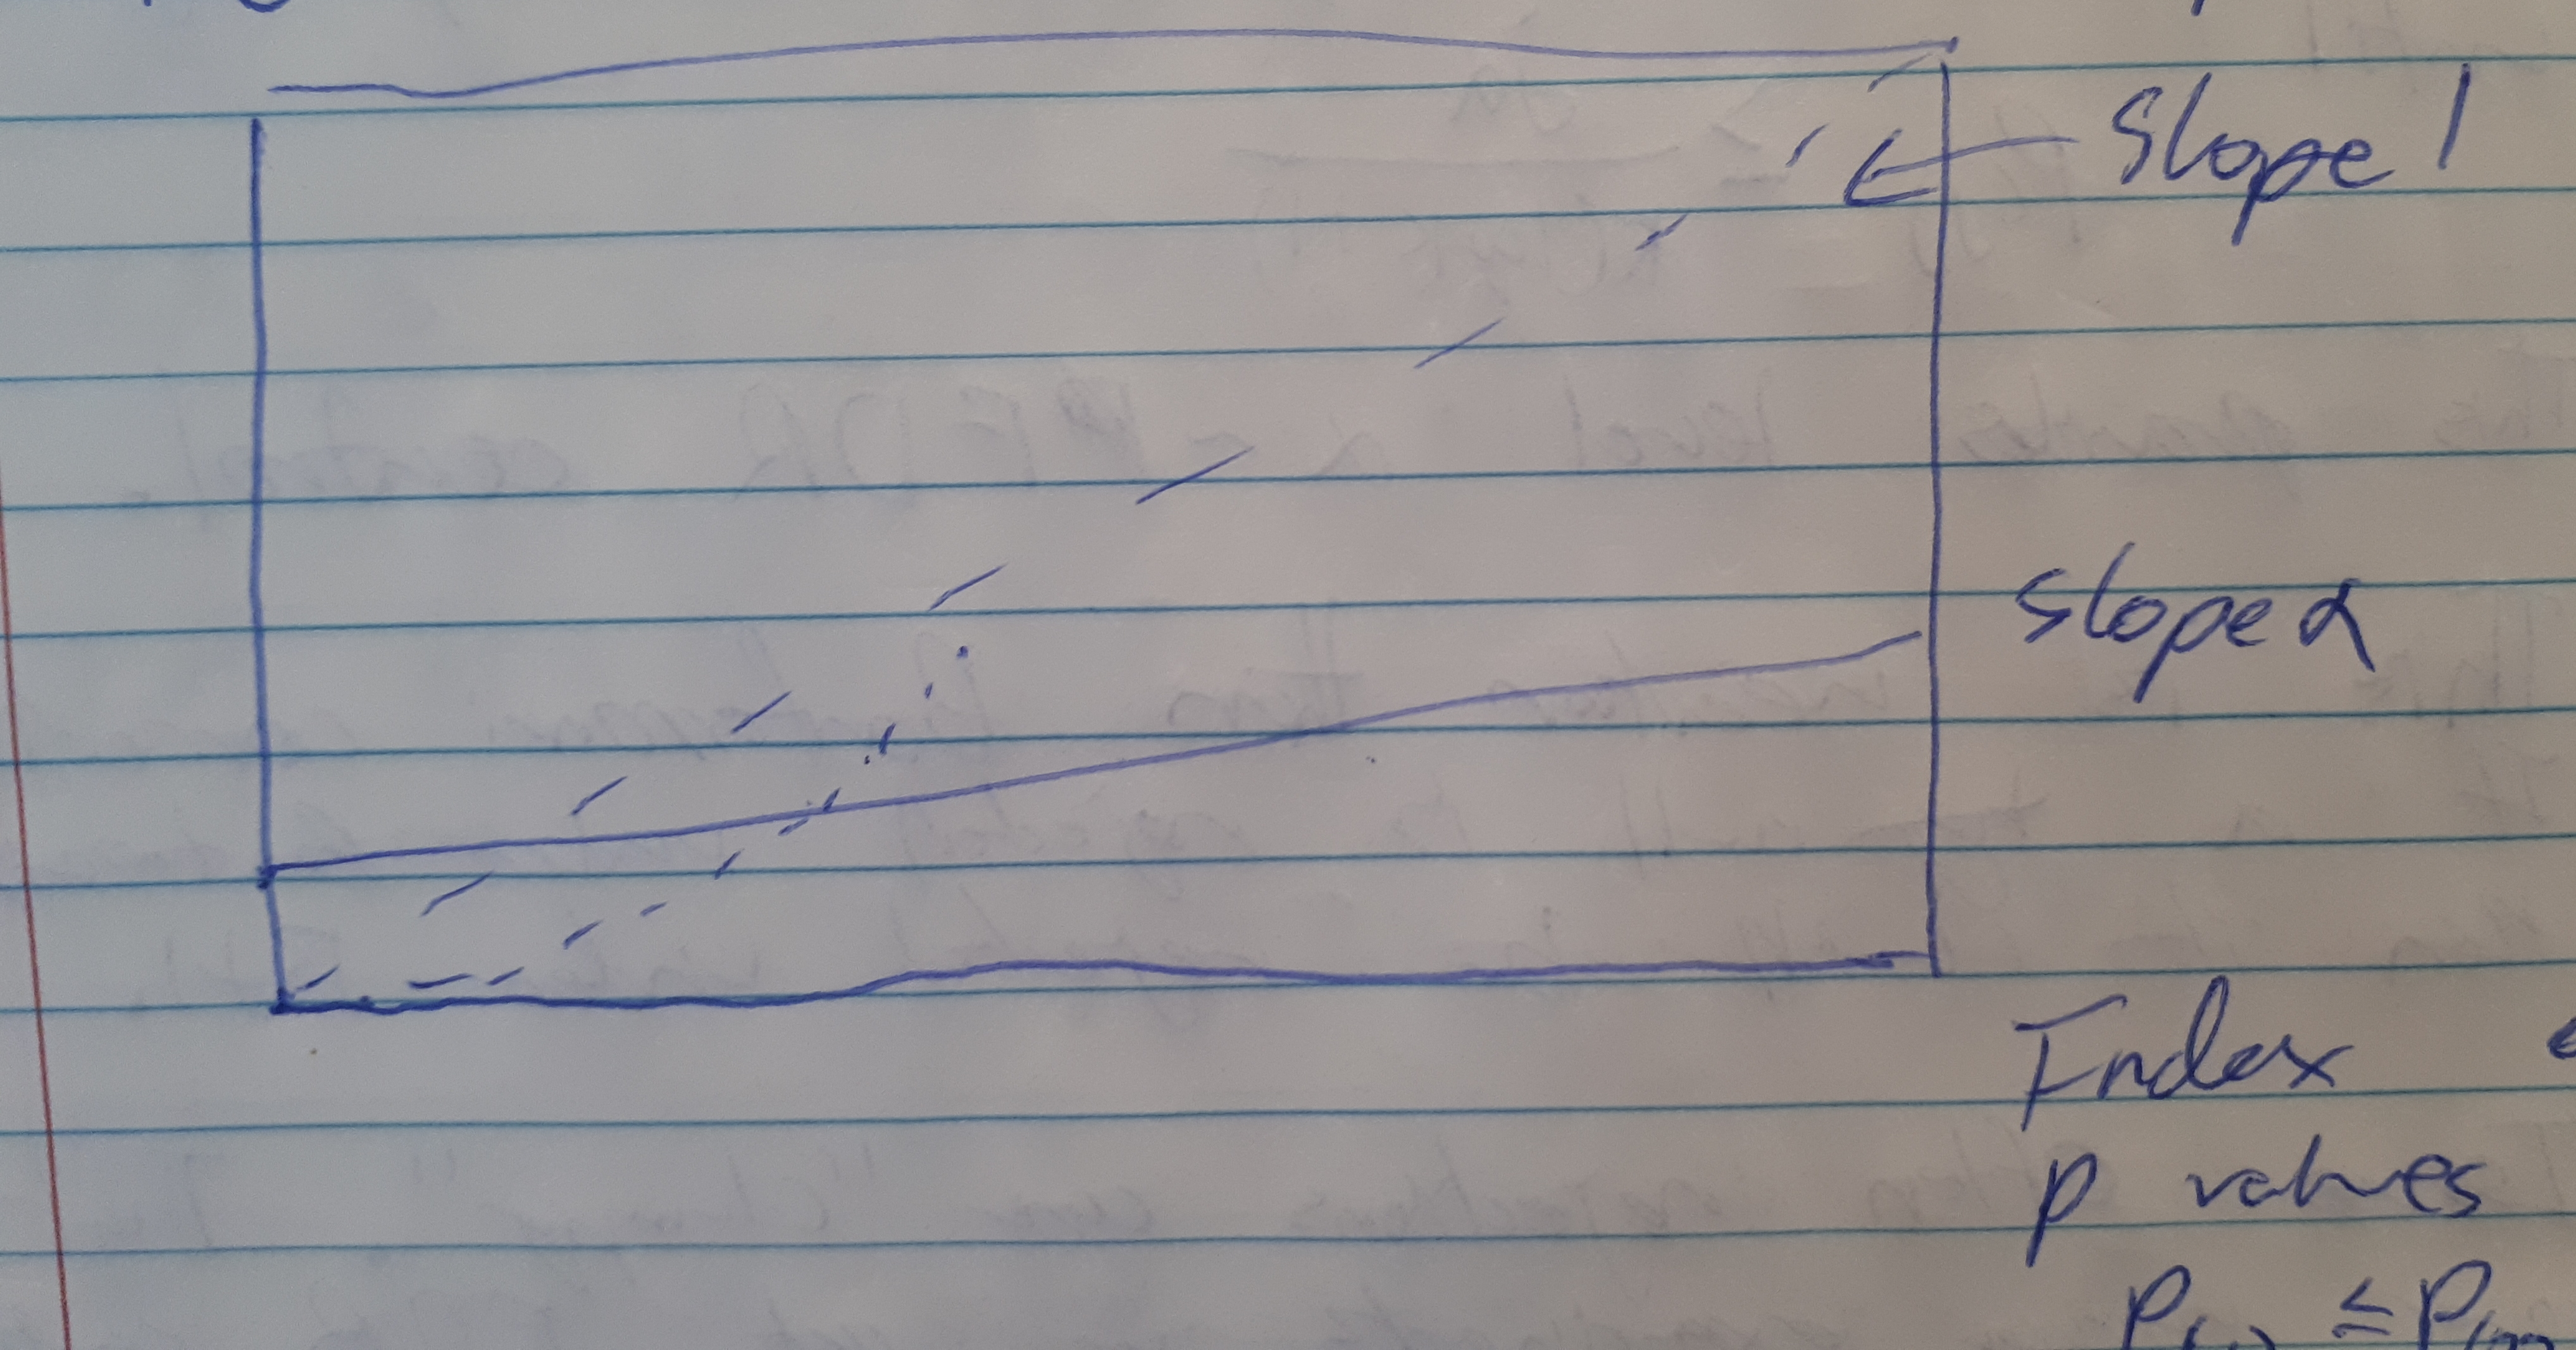
\includegraphics[width = \textwidth]{10_21_P01.jpg}
\end{center}

The Benjamini Hochberg prodecure says to reject until $p_{(j)} \ge \frac{j\al}{k}$.
\begin{thrm}
    \emph{[Benjamini-Hochberg '95]} Let $N_0 = \#$ of true nulls (nulls we shouldn't reject) if the $p$-values are independent, then BH procedure satisfies 
    \[FDR \le \frac{N_0}{k} \al \le \al. \]
    If the $p$-values are dependent, then we always have
    \[FDR \le H(k) \frac{N_0}{k} \al \le H(k)\al, \]
    where $H(k) = 1+\frac{1}{2}+\ldots + \frac{1}{k}$ is the $k^{th}$ harmonic number and satisfies $H(k) \le \log(k)+1$. Thus if we use the strong criterion reject until 
    \[p_{(j)} \ge \frac{j\al}{\log(k)+1}, \]
    then we are guaranteed level $\al$ FDR control.
\end{thrm}
The BH correction is weaker than the Bonferronni correction. If a null is rejected under Bonferroni, then it will still be rejected under BH. Some nulls will be rejected under BH that won't be rejected under Bonferroni.

We still have the issue that often our rejections are ``clumpy''. That is, we only have control over the average FDP over many experiments. We often see in experiments $\{0\%, 0\%, 0\%, 100\%\}$-false rejections which has an average FDP of $25\%$ but obviously sometimes we have far too many false rejections. 

\section{Model diagnostics}
Motivation: when doing a linear model we want to do as well as possible. Thus we often need to
\begin{itemize}
    \item Decide when a fit is ``good enough'' so that the assumptions make sense.
    \item Choose good features/covariates.
\end{itemize}
\subsection{Leverage scores}
Suppose we have the model $Y = X\beta +\eps$. Define $H=X(X^TX)^{-1}X^T$ which is our hat matrix/the orthogonal projection onto the range of $X$. 

We can ask how much does a single example/observation affect our model predictions. That is, what is 
\[\frac{\partial \wh{y}_i}{\partial y_i} = \text{the change in predicted value $\wh{y}_i$ given a change in $y_i$}. \]
We know that $\wh{y}=Hy$. Thus if $H=[H_{ij}]_{i,j=1}^n$, then $\wh{y}_i = \sum_{i=1}^n H_{ij}\wh{y}_j$ and so $\frac{\partial \wh{y}_i}{\partial y_i} = H_{ii}$.
\begin{defn}
    The \emph{leverage score} for example $i$ is $H_{ii}$. (We can interpret this as the self influence of $y_i$ on $\wh{y}_i$).
\end{defn}
Intuition: points with high leverage may actually be problematic as estimates depend strongly on them (although whether or not they are problematic depends on the situation).

Note that

\begin{equation}\label{ge0}
    H_{ii}(1-H_{ii}) = \sum_{j\neq i}H_{ij}^2 \ge 0.
\end{equation}

Thus $H_{ii} \in [0,1]$. Also we have
\[\sum_{i=1}^n H_{ii} = \tr(H) = \tr(X(X^TX)^{-1}X^T) = \tr(X^TX(X^TX)^{-1}) =\tr(I_d) = d. \]
Thus if $H_{ii} \ge \frac{2d}{n}$ (or $\frac{3d}{n}$), then the leverage score of $i$ is high (since it is higher than the average $d/n$). To see equation \eqref{ge0} is true recall that $H^2=H$ and $H^T = H$. Thus
\[H=H^2 =H^TH = (h^T_jh_i)_{i,j=1}^n, \]
where $H=[h_1,\ldots, h_n]$. Thus 
\[ H_ii = h_i^Th_i = \sum_{j=1}^n H_{ij}^2.\]
Thus $H_ii - H_{ii}^2 = \sum_{j\neq i} H_{ij}^2$, as claimed.

\begin{defn}
    Given a symmetric matrix $A \succ 0$ (ie $A^T=A$ and $A$ is positive definite). Define $\norm{x}_A^2 := x^TAx$ to be the \emph{Mahalanobis norm}. We can then define $D(x,y) = \norm{x-y}_A$ to be the \emph{Mahalanobis distance}.
\end{defn}
The Mahalanobis norm measures distances scaled by an ellipse. If $A= \sum_{i=1}^d \la_i(A)u_iu_i^T$, then the set $\{v : v^TA^{-1}v \le 1 \}$ is an ellipse with principal axes $u_i$ with length $\sqrt{\la_i(A)}$ (see picture).

\begin{center}
    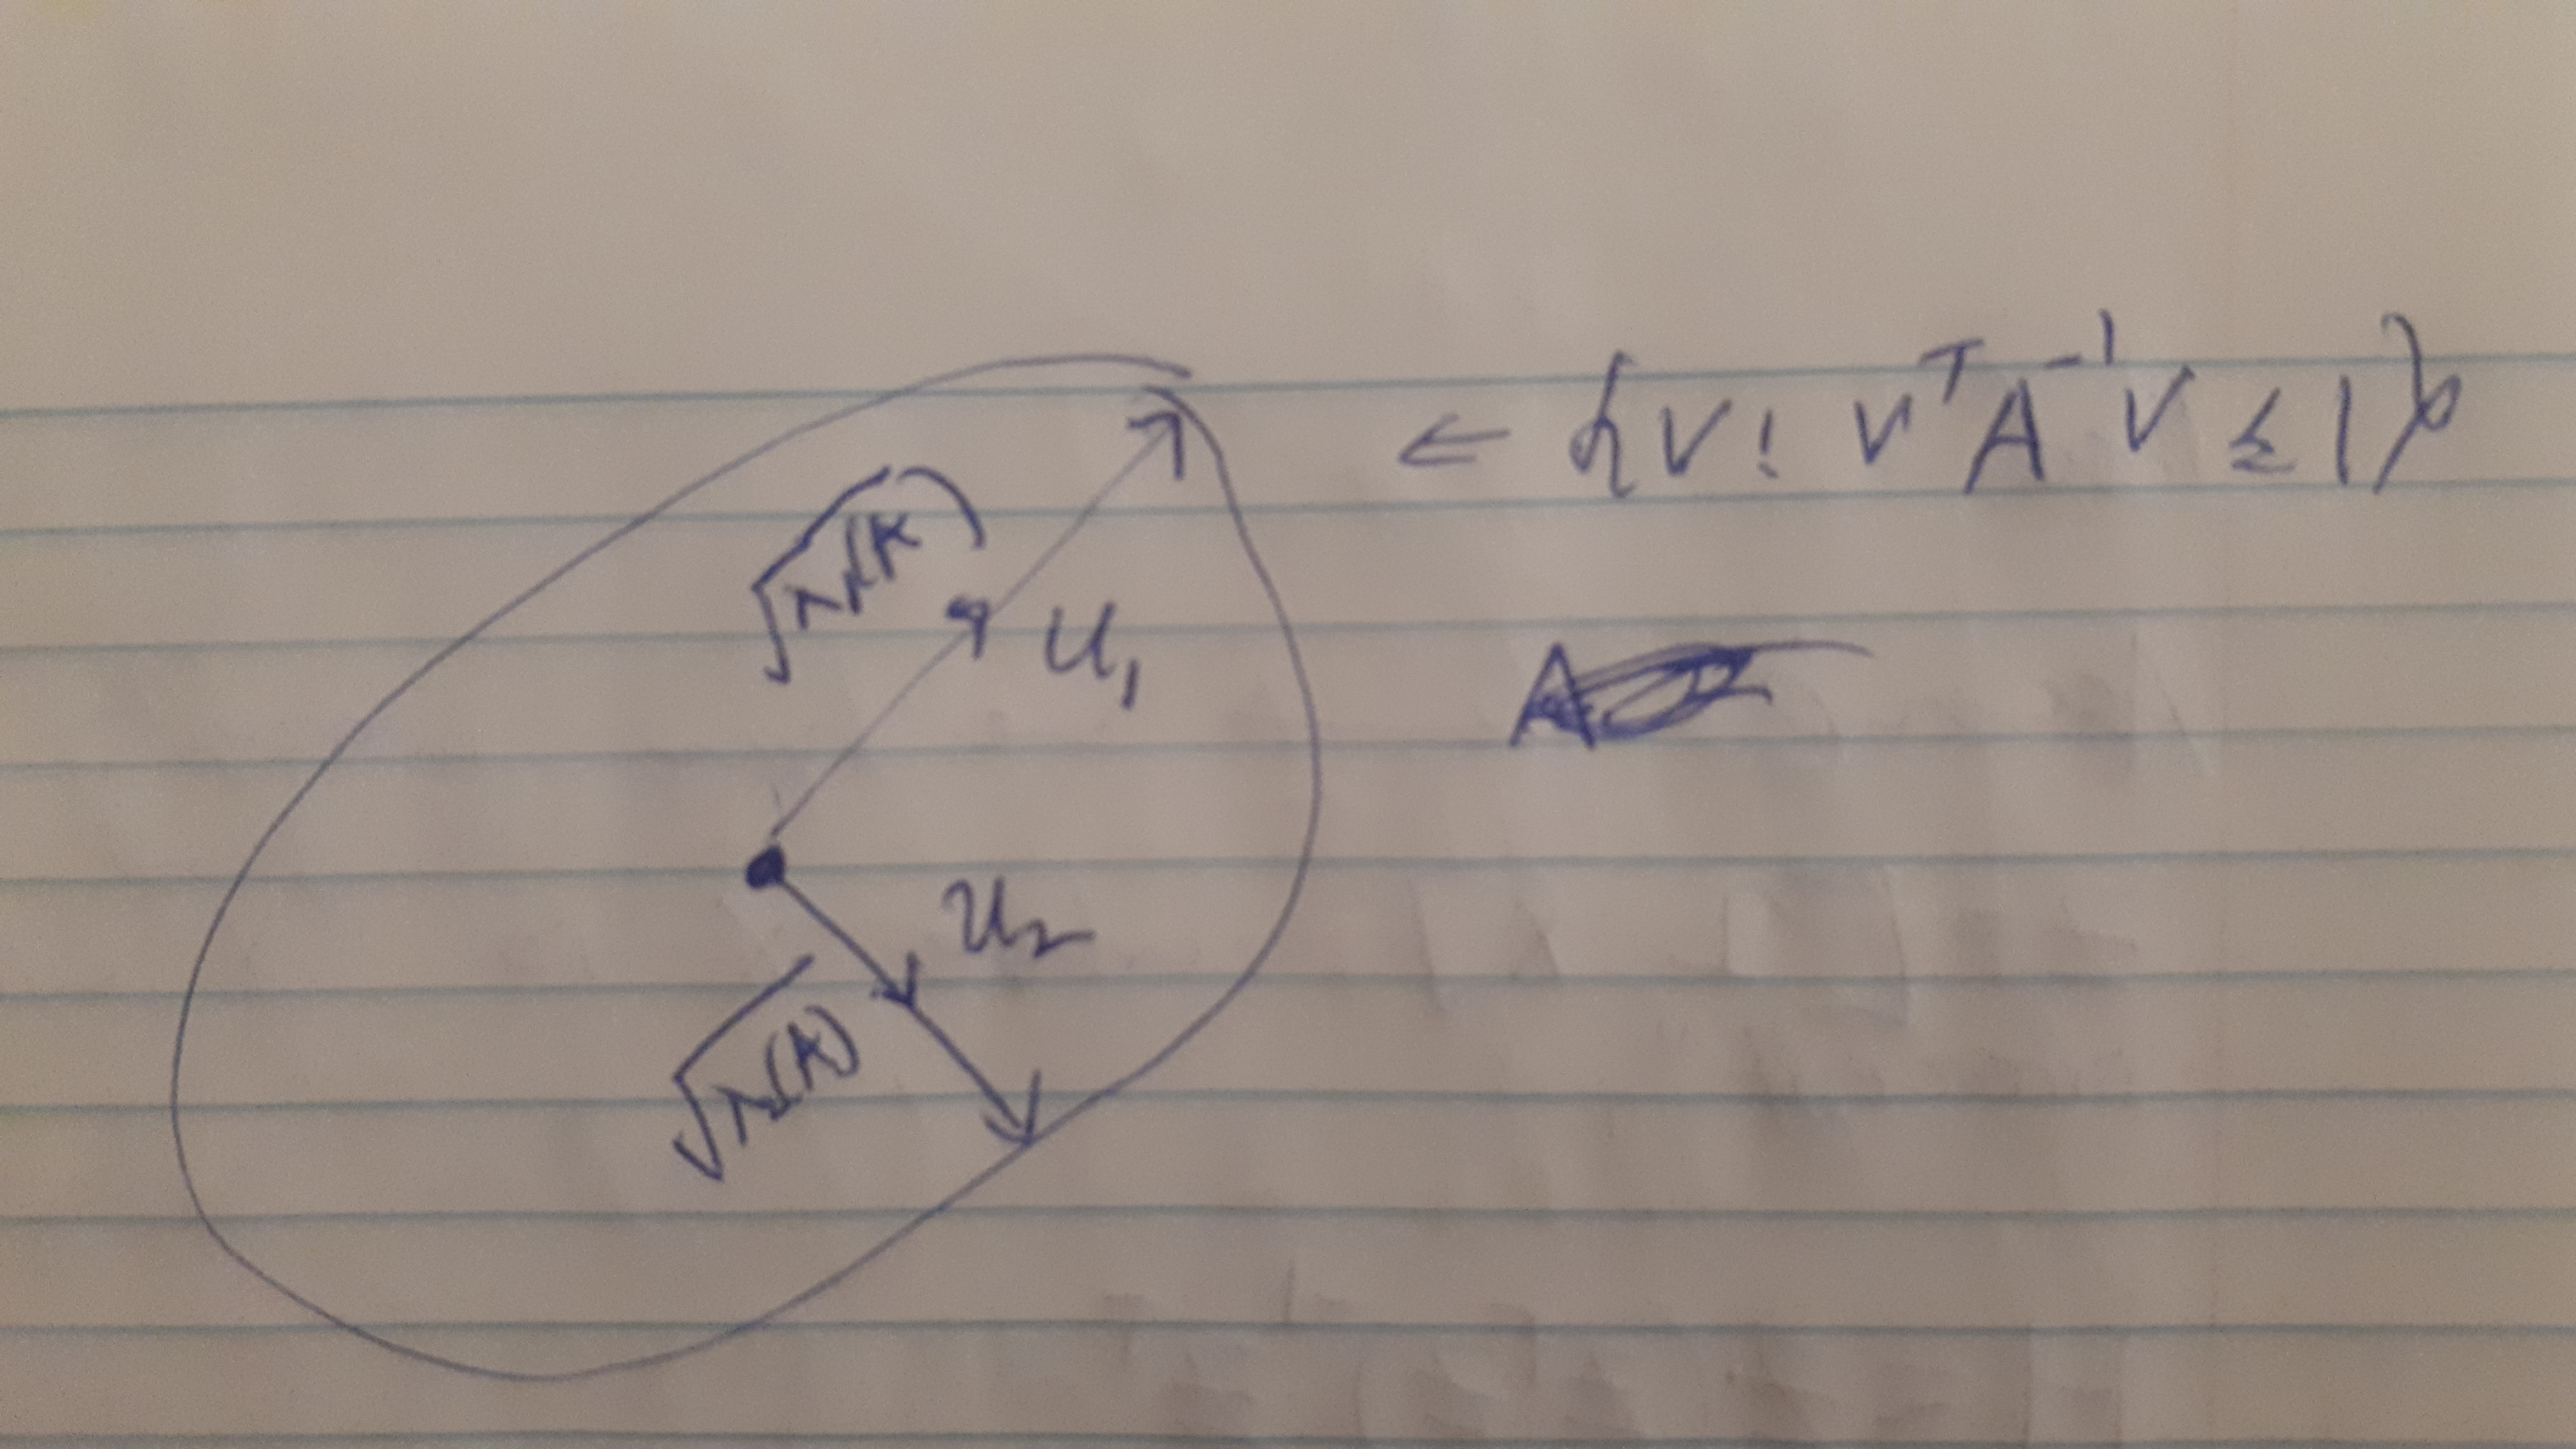
\includegraphics[width = \textwidth/2]{10_21_P02.jpg}
\end{center}

Consider now a pile of data points $x_i$ and let $\bar{x}_n =\frac{1}{n}\sum_{i=1}^n x_i$ and define the sample covariance to be $S=\frac{1}{n}\sum_{i=1}^n(x_i-\bar{x}_n)(x_i-\bar{x}_n)^T$. The matrix $S$ tells us the shape of the ``bulk'' of our data. See picture:

\begin{center}
    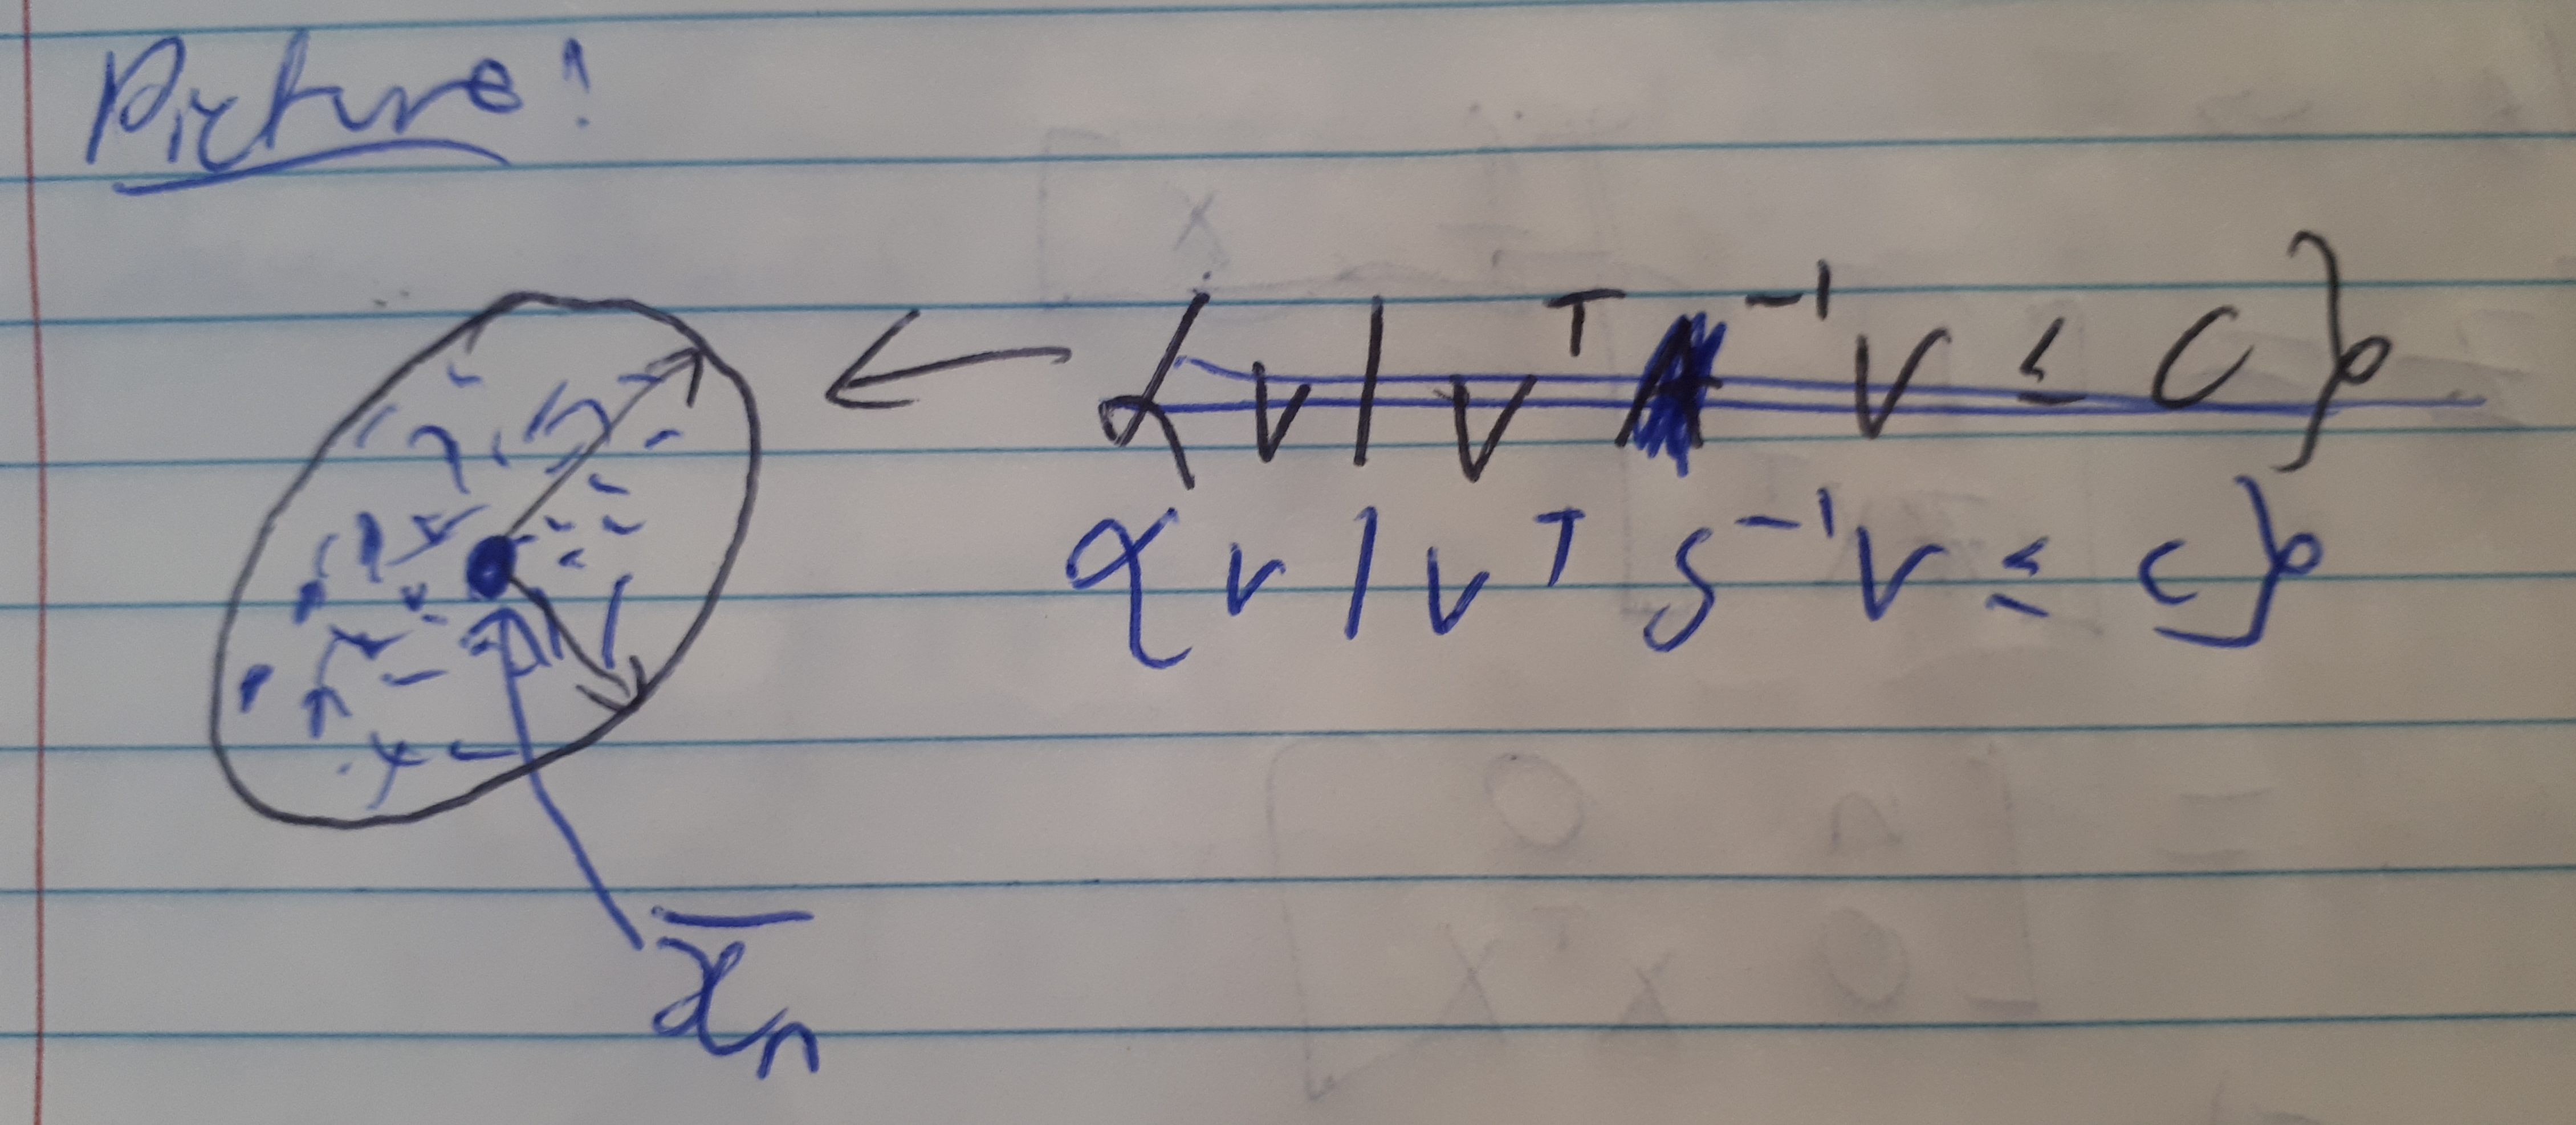
\includegraphics[width = \textwidth/2]{10_21_P03.jpg}
\end{center}

For $x \in \R^d$, define 
\[D^2(x) = (x-\bar{x}_n)^TS^{-1}(x-\bar{x}_n). \]
Thus $D^2(x)$ is a measurement of how far $x$ is from the ``bulk'' of our data set.
\begin{prop}
    If the data has an intercept term, then $D^2(x_i) = nH_{ii}-1$.
\end{prop}
\begin{proof}
    Since we have an intercept write $Z=[\one, X]$ where $X$ is ``$X$ without the intercept''. Define $H=Z(Z^TZ)^{-1}Z^T$. Since our data has an intercept we can assume without loss of generality that $\bar{x}_n = \frac{1}{n}X^T\one = 0$. This implies that
    \begin{align*}
        Z^TZ &= \begin{bmatrix}
            \one^T\\X^T
        \end{bmatrix}[\one, X]\\
        &=\begin{bmatrix}
            n&0\\
            0&X^TX
        \end{bmatrix}.
    \end{align*} 
    Thus 
    \[(Z^TZ)^{-1} = \begin{bmatrix}
        \frac{1}{n}&0\\
        0&(X^TX)^{-1}
    \end{bmatrix}, \]
    and 
    \[H = [\one, X]\begin{bmatrix}
        \frac{1}{n}&0\\
        0&(X^TX)^{-1}
    \end{bmatrix}\begin{bmatrix}
        \one^T\\X^T
    \end{bmatrix}.\]
    Write 
    \[X=\begin{bmatrix}
        x_1^T\\ \vdots \\ x_n^T
    \end{bmatrix}~~ \text{and} ~~
    X^T = [x_1,\ldots, x_n]. \]
    The diagonal entries of $H$ are thus
    \[H_{ii}= [1, x_i^T]\begin{bmatrix}
        \frac{1}{n}&0\\
        0&(X^TX)^{-1}
    \end{bmatrix}\begin{bmatrix}
        1\\x_i
    \end{bmatrix} =\frac{1}{n}+x_i^T(X^TX)^{-1}x_i. \]
    Note that since $\bar{x}_n = 0$,
    \begin{align*}
        H_{ii}&=\frac{1}{n}+x_i^T(X^TX)^{-1}x_i\\
        &=\frac{1}{n}\left(1 + nx_i^T(X^TX)^{-1}x_i\right)\\
        &=\frac{1}{n}\left(1 + x_i^T(\frac{1}{n}X^TX)^{-1}x_i\right)\\
        &=\frac{1}{n}\left(1 + (x_i-\bar{x}_n)^T\left(\frac{1}{n}X^TX-\bar{x}_n\bar{x}_n^T\right)^{-1}(x_i-\bar{x}_n)\right)\\
        &=\frac{1}{n}\left(1 + (x_i-\bar{x}_n)^TS^{-1}(x_i-\bar{x}_n)\right)\\
        &=\frac{1}{n}(1+D^2(x_i)).
    \end{align*}
    Thus $D^2(x_i) = nH_{ii}-1$.
\end{proof}
Thus high leverage corresponds to the distance of $x_i$ from the bulk of the data. Consider the following picture:

\begin{center}
    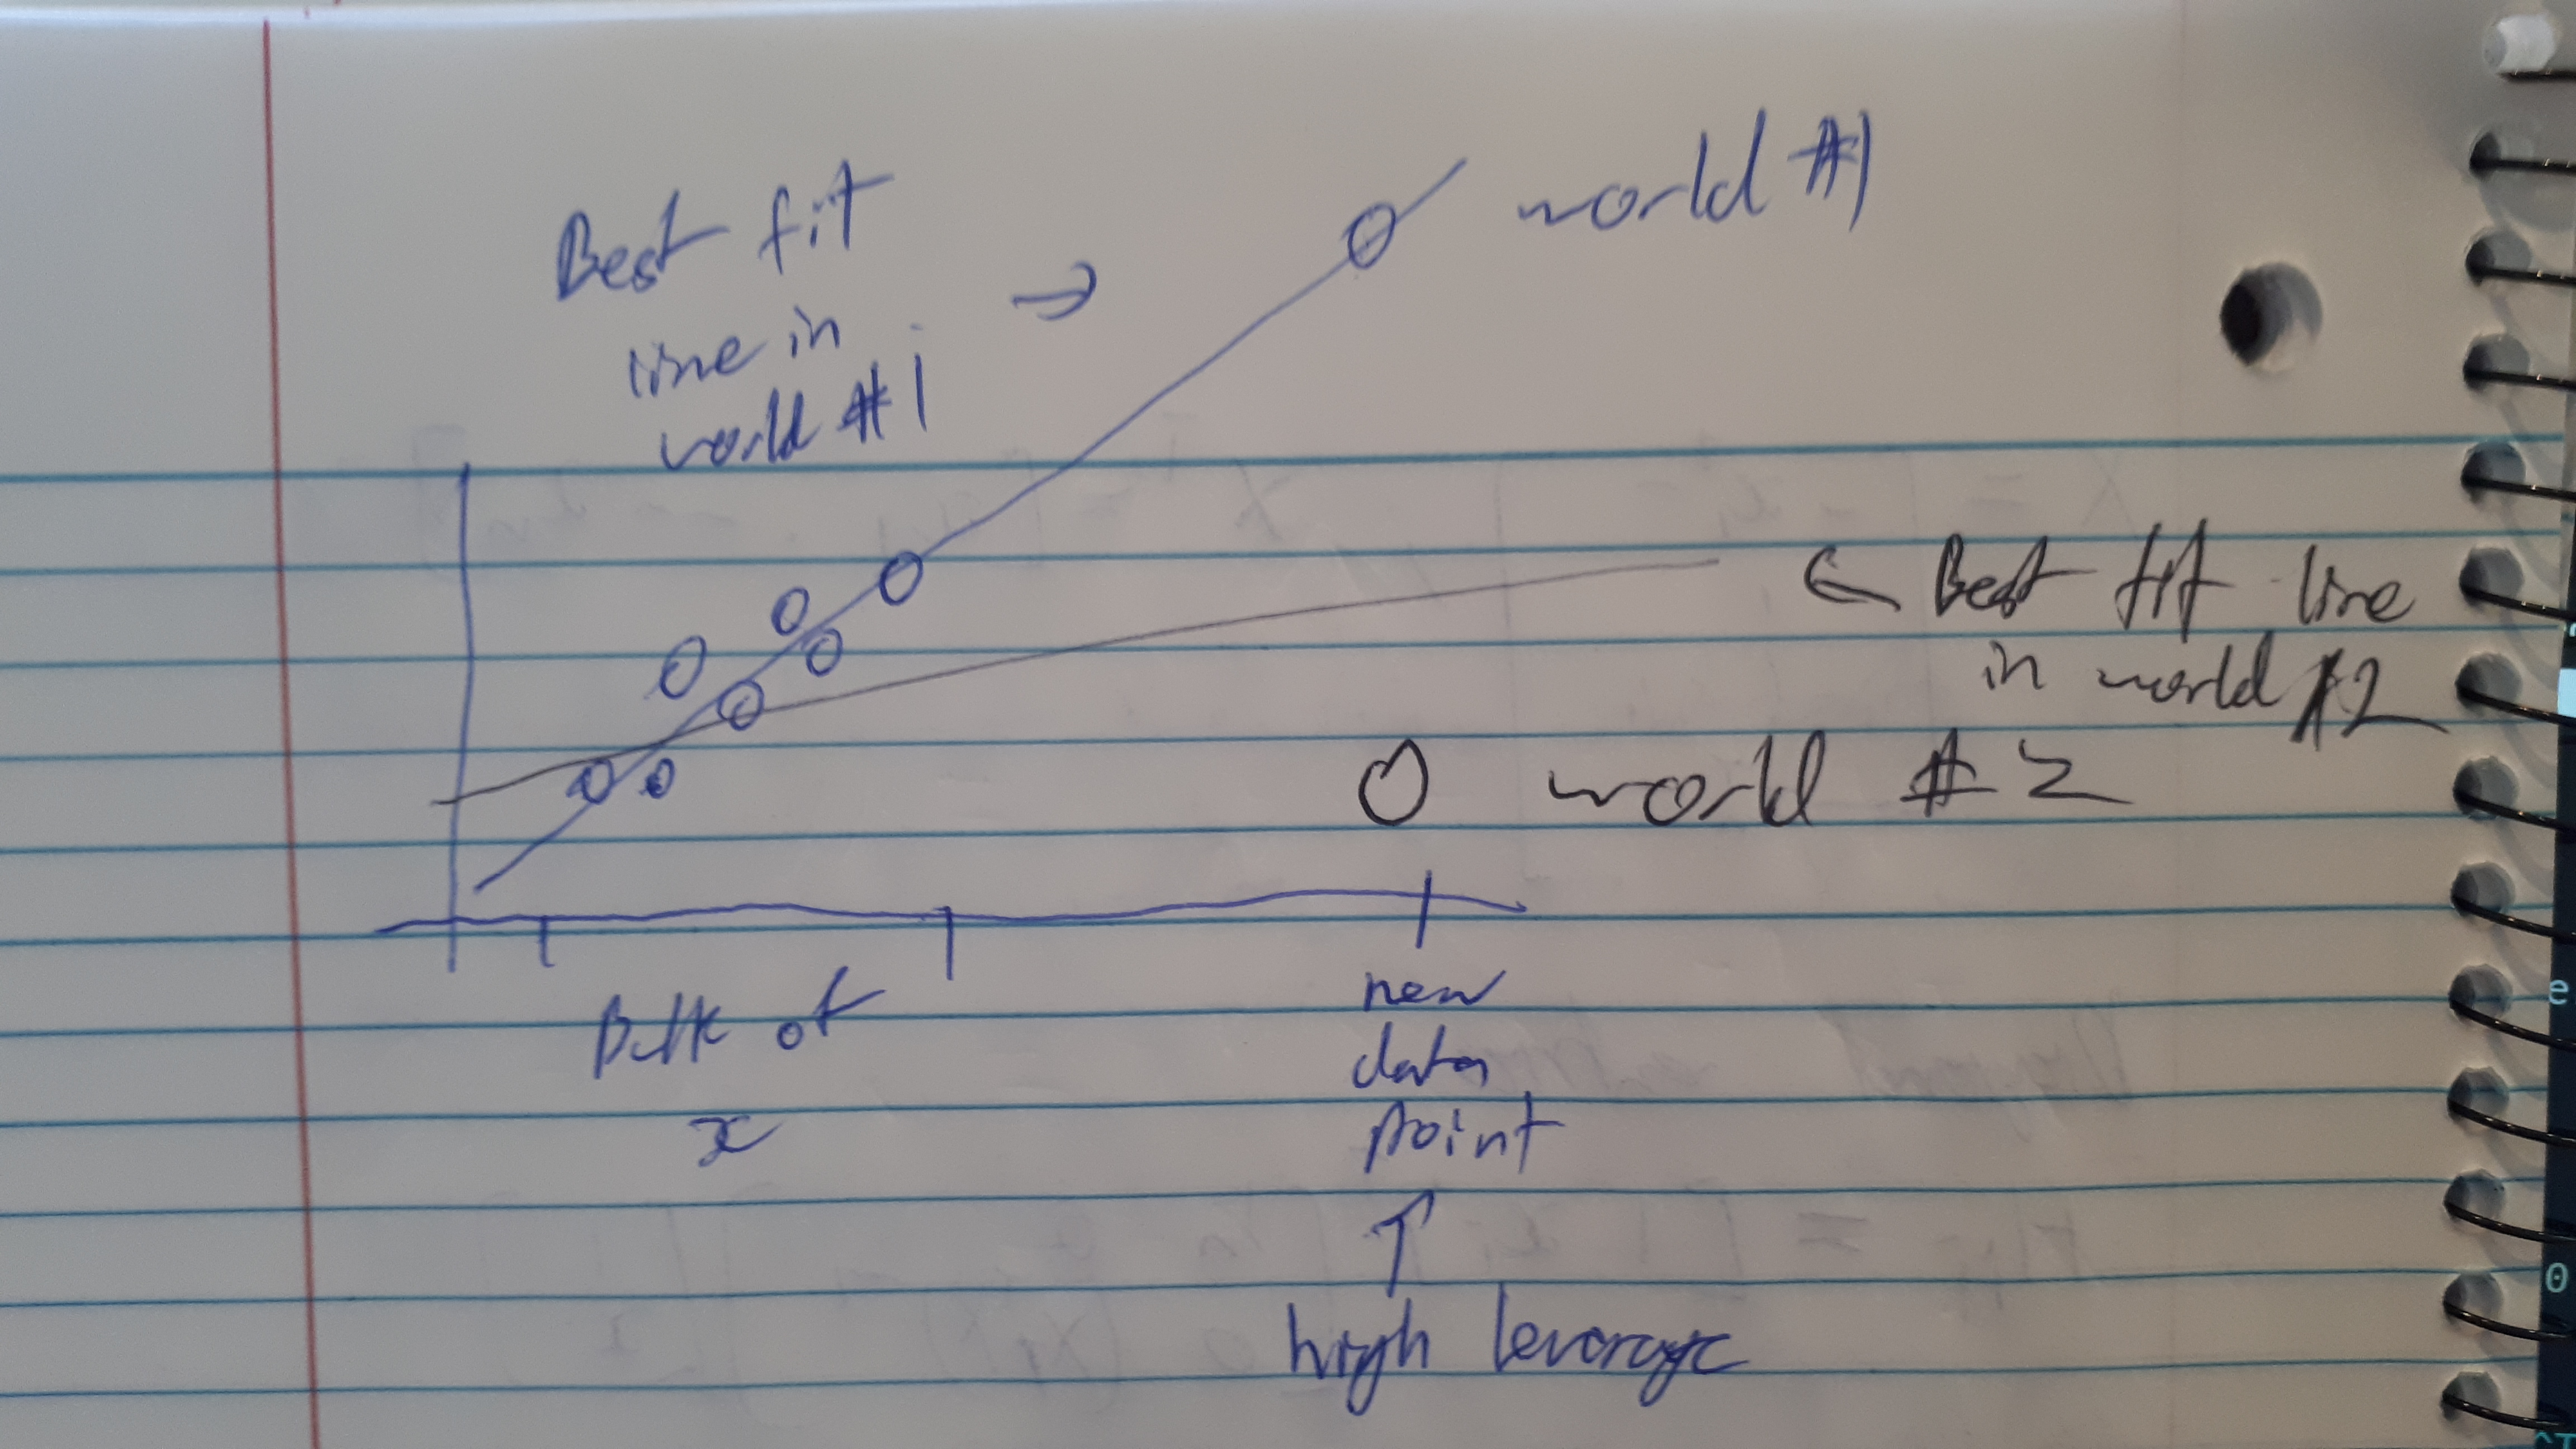
\includegraphics[width = \textwidth]{10_21_P04.jpg}
\end{center}

In this picture, the bulk of our data is quite tightly clustered. Consider adding a much larger new data point $x_i$. This is a point of high leverage by the proposition. We can now consider two worlds corresponding to two different choices of $y_i$. We have world \#1 where the new $y_i$ matches the trend of the rest of the data points. We could also have world \#2 where the new data point is far from the trend of the rest of the data.

In both of these world we can make a line of best fit. In world \#1  the new point is good and it nails down the slope and suggests our model is good. In model \# 2 the new point is not so good. It drastically changes our model. When we have data points like in world \# 2 we have to consider two possibilities. It might be the case that the new data point is an outlier due to measurement error. In this case we should consider removing it. If we are very sure of our measurements for the new data, then this will suggest that the model is not correct and we should not just chuck out the new point.

\section{Leave one out predictions}
Idea: the error in prediction $y_i$ from all data except $i$ should have more ``fidelity'' to the real world.

\begin{notn}
    Let $H=X(X^TX)^{-1}X^T$, 
    \[y_{\setminus i} = \begin{bmatrix}
        y_1\\\vdots\\ y_{i-1} \\ y_{i+1} \\ \vdots \\ y_n
    \end{bmatrix} \in \R^{n-1},\]
    and
    \[X_{\setminus i} = \begin{bmatrix}
        x_1^T\\\vdots\\ x_{i-1}^T \\ x_{i+1}^T \\ \vdots \\ x_n^T
    \end{bmatrix} \in \R^{(n-1)\times d}. \]
    Also define $\wh{\beta}_{\setminus i} = (X_{\setminus i}^TX_{\setminus i})^{-1}X^T_{\setminus i}y_{\setminus i}$. Thus all of these correspond to the model when we remove $y_i$. Lastly define $\wh{y}_{\setminus i} = x_i^T\wh{\beta}_{\setminus i}$ which is the predicted $y$-value for $x_i$ without using $(x_i, y_i)$. 
\end{notn}
\begin{prop}
    With the notation as above, $\wh{y}_i = H_{ii}y_i+(1-H_{ii})\wh{y}_{\setminus i}$.
\end{prop}
\begin{proof}
    Recall the Sherman-Morrison-Woodbury identity (proved on homework)
    \[(A-uu^T)^{-1}  = A^{-1}+\frac{A^{-1}uu^TA^{-1}}{1-u^TA^{-1}u},\]
    where $A$ is a matrix and $u$ is a vector. Note that 
    \[X_{\setminus i}^T X_{\setminus i} =X^TX - x_ix_i^T. \]
    Set $M=X^TX$, then 
    \[(X_{\setminus i}^TX_{\setminus i})^{-1} = M^{-1}+\frac{M^{-1}x_ix_i^TM^{-1}}{1-x_i^TM^{-1}x_i}. \]
    Observe that $x_iM^{-1}x_j = H_{ij}$. Now consider $\wh{y}_i$ and $\wh{y}_{\setminus i}$. We have
    \[\wh{y}_i = (Hy)_i = H_{ii}y_i + \sum_{j\neq i}H_{ij}y_j. \]
    And,
    \begin{align*}
        \wt{y}_{\setminus i}&=x_i^T \wh{\beta}_{\setminus i}\\
        &= x_i^T(X_{\setminus i}^TX_{\setminus i})^{-1}X_{\setminus i}^Ty_{\setminus i}\\
        &=x_i^T\left(M^{-1}+\frac{M^{-1}x_ix_i^TM^{-1}}{1-x_i^TM^{-1}x_i}\right)X_{\setminus i}^Ty_{\setminus i}\\
        &=x_i^TM^{-1}X_{\setminus i}^Ty_{\setminus i}+\frac{(x_iM^{-1}x_i)(x_i^TM^{-1}X_{\setminus i}^T y_{\setminus i})}{1-x_i^TM^{-1}x_i}.
    \end{align*}
    Note that since $H_{ij} = x_j^TM^{-1}x_i$, we have $x_i^TM^{-1}x_i = H_{ii}$ and
    \[X^T_{\setminus i}(X^TX)^{-1}x_i = [H_{ij}]_{j\neq i}.\]
    And so
    \[x_i^T(X^TX)^{-1}X_{\setminus i}^Ty_{\setminus i} = \sum_{j \neq i}H_{ij}y_j. \]
    Subsituting this we have
    \begin{align*}
        \wh{y}_{\setminus i}=&\sum_{j \neq i}H_{ij}y_j+\frac{H_{ii}\sum_{j\neq i}H_{ij}y_j}{1-H_{ii}}\\
        =&\left(\frac{1-H_{ii}}{1-H_{ii}}+\frac{H_{ii}}{1-H_{ii}}\right)\sum_{j\neq i} H_{ij}y_j\\
        =&\frac{1}{1-H_{ii}}\sum_{j\neq i} H_{ij}y_j.
    \end{align*}
    Thus $(1-H_{ii})\wh{y}_{\setminus i} = \sum_{j\neq i}H_{ij}y_j$. Subsituting this into our formula for $\wh{y}_i$ we can conclude that 
    \[\wh{y}_i = H_{ii}y_i + (1-H_{ii})\wh{y}_{\setminus i}.\qedhere \]
\end{proof}
\end{document}